\chapter{Analytics Application}\label{ch5:expl_applied}

\section{Data Modeling}

\begin{wrapfigure}{R}{0.45\linewidth}
\centering
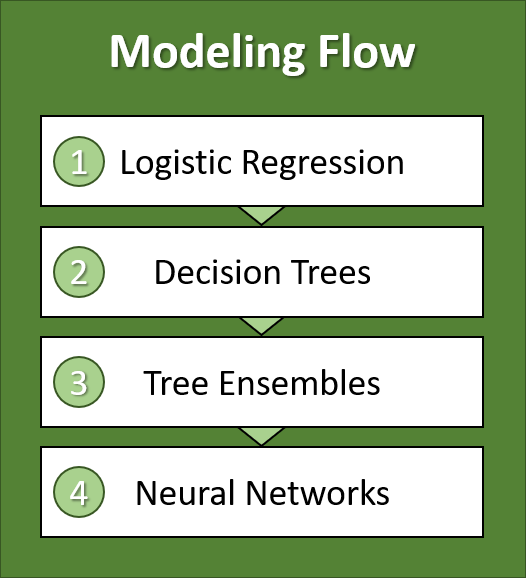
\includegraphics[scale=.6]{templates/images/Flow-Modeling.png}
\singlespacing
\caption[Modeling workflow]{Workflow for predicting the class of geothermal gradient across the southwestern NM study area using a variety of common machine learning methods.}
\label{fig:model_flow}
\end{wrapfigure}

Supervised learning methods for classification come in a wide variety of shapes and sizes. Rather than settle on one for predicting geothermal gradient, four different methods are applied to the southwestern NM data set. Figure \ref{fig:model_flow} illustrates the high-level modeling flow, where model complexity increases with successive steps. The method descriptions below only briefly delve into important model mechanics and key hyperparameters (i.e., parameters not learned from data) that impact model performance. Other sources can provide a deeper review of machine learning algorithms and their mathematical underpinnings. This investigation should instead be considered an applied case study that uses these algorithms as tools for generating insights on geothermal potential. 

\subsection{Assessing Performance}
Building an intuition for the differences in predictive ability of different models first requires a clear definition of the scoring metric(s) used to compare those models. The characterization of classifier performance typically begins with a confusion matrix. In its simplest form, the confusion matrix evaluates class predictions as \acrlong{tp} (\acrshort{tp}; predicted 1, actually 1), \acrlong{tn} (\acrshort{tn}; predicted 0, actually 0), \acrlong{fp} (\acrshort{fp}; predicted 1, actually 0), and \acrlong{fn} (\acrshort{fn}; predicted 0, actually 1). For the multi-class problem, the confusion matrix expands to include all correct classification and mis-classification options. Figure \ref{fig:confusion_matrix} illustrates the elements of a 4-class matrix.

\begin{figure}[!htp]
\centering
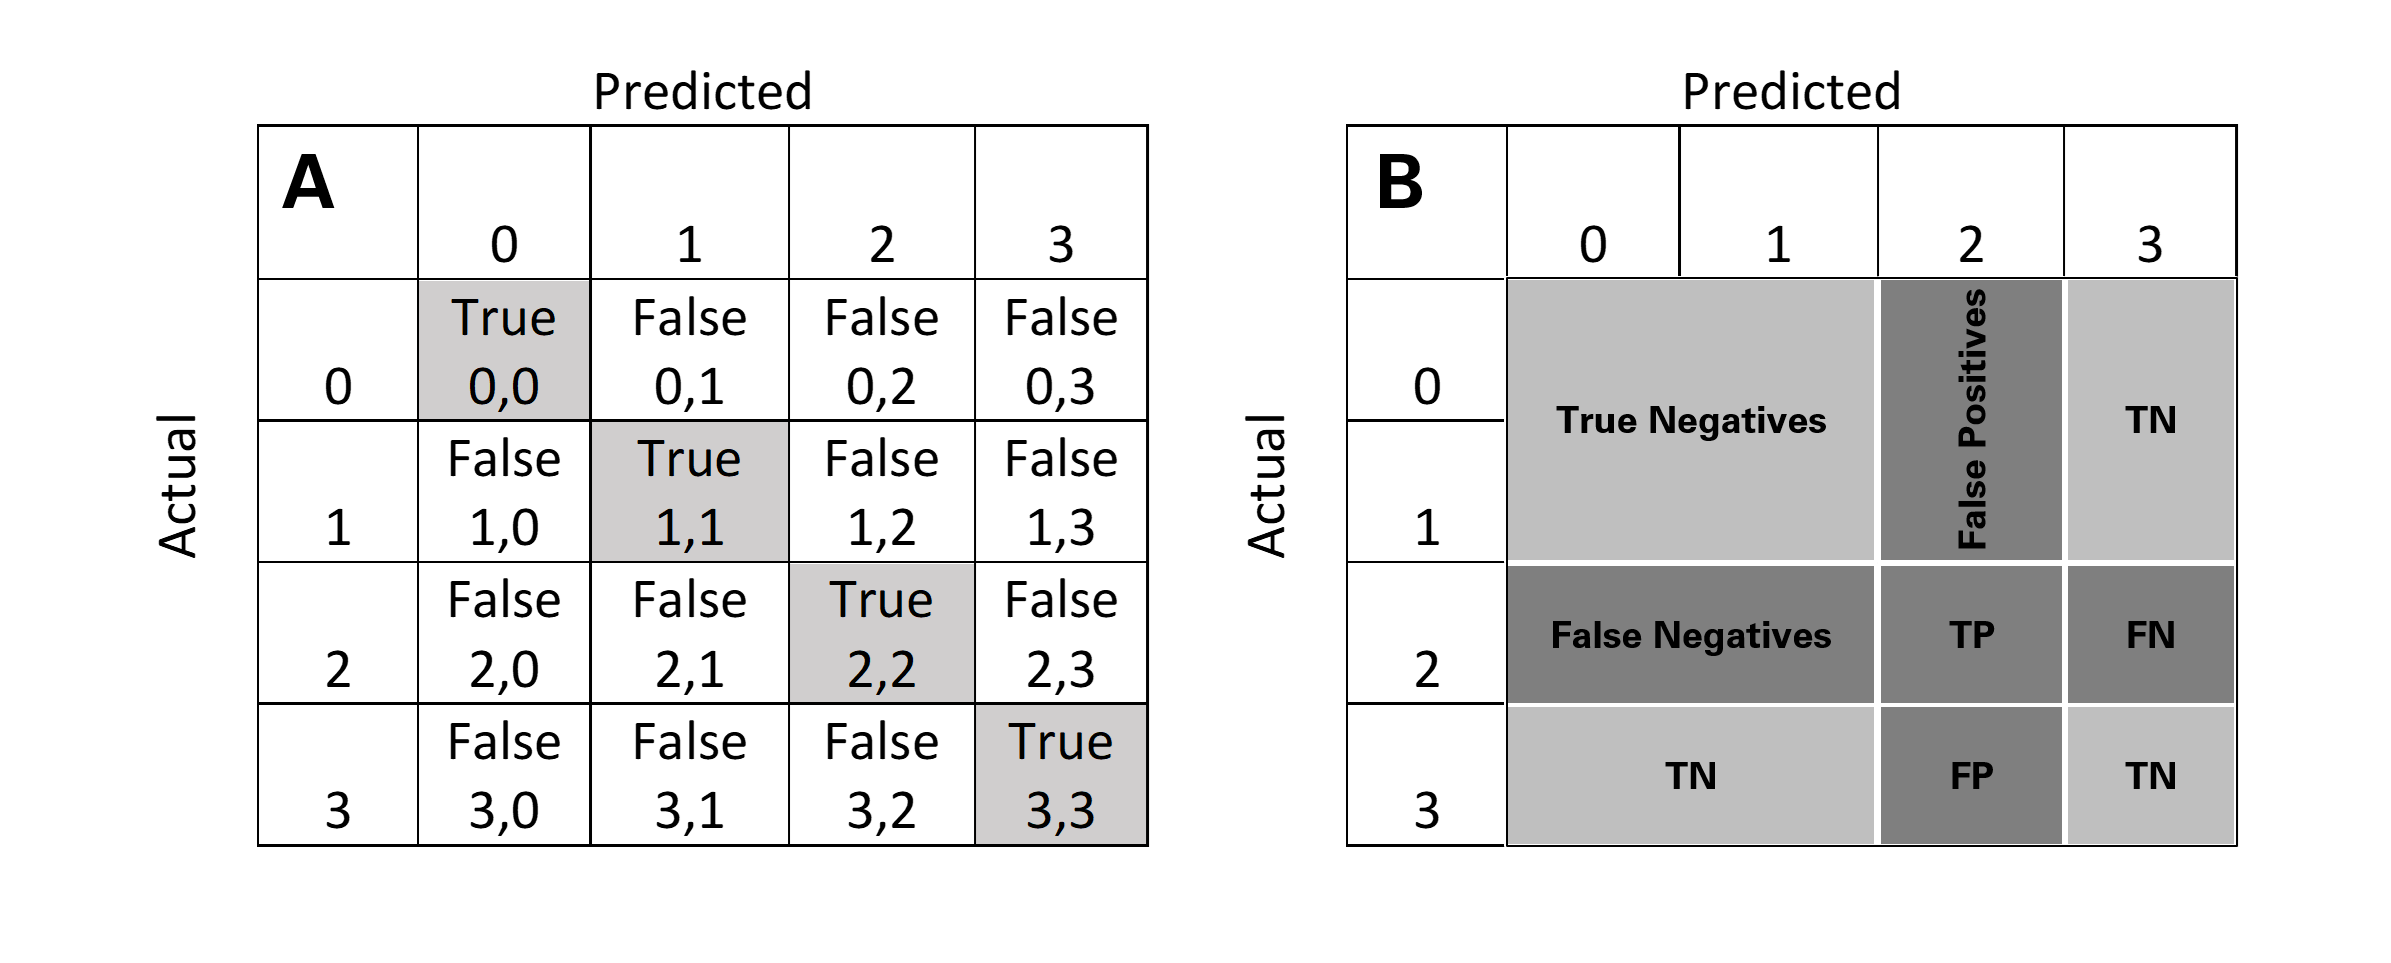
\includegraphics[width=\textwidth]{templates/images/Figure-Confusion_Matrix.png}
\caption[Four-class confusion matrix]{Confusion matrix diagram for a 4-class scenario. A. Each cell represents a pairing between an actual class label (rows) and the predicted label (columns). True positives for each class are down the diagonal. B. Example of matrix interpretation using class 2 as a point of reference. Elements associated with TP, FP, TN, and FN values are labeled.}
\label{fig:confusion_matrix}
\end{figure}

Several statistical measures can be defined using combinations of elements in the confusion matrix. Of significance to this study are the \acrlong{tpr} (\acrshort{tpr}) and \acrlong{fpr} (\acrshort{fpr}) \citep{tharwat_classification_2020}:

\begin{itemize}
\item \textbf{True Positive Rate}: the count of correctly-predicted positives scaled by the actual positives: TP/(TP$+$FN).
\item \textbf{False Positive Rate}: the count of incorrectly-predicted positives scaled by the actual negatives: FP/(FP$+$TN).
\end{itemize}

Classification relies on a probability threshold for assigning a class label. As the threshold lowers, the chances the classifier will believe it has a label match will increase. By varying this threshold, it becomes possible to map out the discriminating ability of a classifier by plotting a curve in TPR vs. FPR space (Figure \ref{fig:roc}). This is commonly referred to as the \acrlong{roc} (\acrshort{roc}) curve \citep{fawcett_introduction_2006}. A classifier that cannot discriminate between classes will perform no better than random guessing, resulting in a curve that plots along the diagonal from the origin to the upper right of the plot. On the other hand, a perfect classifier will have a TPR of 1.0 for all thresholds, so it plots straight up along the y-axis and then horizontally at TPR = 1.0. Typical ROC curves plot in the upper-left space between these two extremes.

\begin{figure}[!htp]
\centering
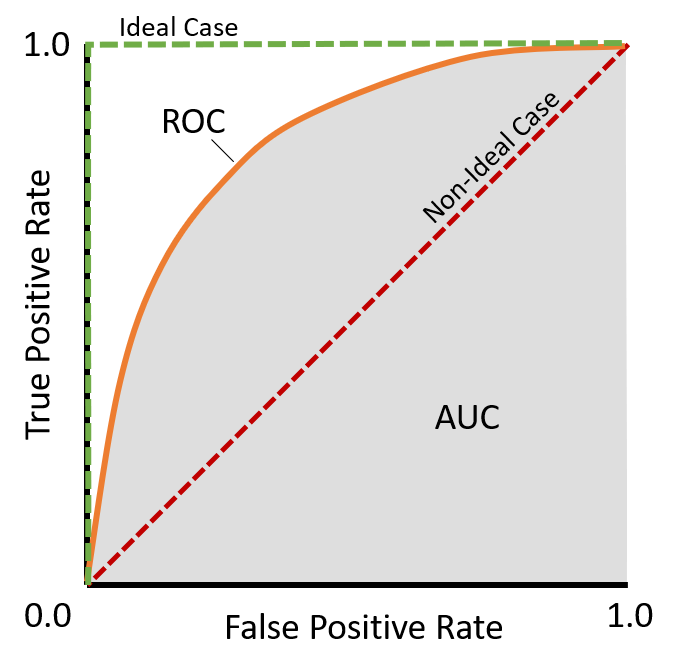
\includegraphics[width=0.5\textwidth]{templates/images/Figure-ROC_AUC_Diagram.png}
\caption[Receiver Operating Characteristic diagram]{ROC curve diagram in TPR vs. FPR space. Perfect classifiers will plot along the ideal case line (green), poor classifiers plot along the diagonal (red). AUC (gray) characterizes the quality of the classifier on a scale of 0.5 to 1.0.}
\label{fig:roc}
\end{figure}

Area Under the ROC Curve (AUC) defines a summary statistic for the ROC function (see Figure \ref{fig:roc}) \citep{fawcett_introduction_2006}. Since the ideal classifier has a TPR of 1.0 at all times, the ideal AUC also equals 1.0. In the non-ideal case, the AUC drops to 0.5. AUC values and ROC curves provide a standardized means of comparing classifiers and are the primary performance metric used in this thesis.

With multi-class classification, defining single class performance using the definitions of TP, FP, TN, and FN as shown in Figure \ref{fig:confusion_matrix}B is relatively straight-forward. Overall classifier performance across all classes can also be characterized with a single ROC curve using macro, weighted, or micro averaging \citep{scikit-learn_sklearnmetricsroc_auc_score_2021}.

\begin{itemize}
    \item \textbf{Macro}: averaging matches the unweighted arithmetic mean of metric values.
    \item \textbf{Weighted}: averaging follows the procedure of macro-averaging but adds a weight for each class contribution based on the fraction of total observations that fall within that class. 
    \item \textbf{Micro}: averaging considers class results in aggregate, so statistics are calculated across the entire confusion matrix. TPR becomes the accuracy and FPR becomes the error rate.
\end{itemize}

For imbalanced data sets, micro will indicate better performance than macro due to the impact of the dominant class. Both micro and macro averages are included in the classification analysis in the following sections.

\subsection{Logistic Regression} \label{ch5:log_reg}

\subsubsection{Binary Formulation} 

The classic \acrlong{lr} (\acrshort{lr}) model is a binary classifier that predicts one of two labels based on the input data. LR frames the problem as a linear combination of the input observations \citep[~p 369]{bertsimas_analytics_2016}:

\begin{equation}
\label{eq:logreg_form}
    y = W^TX = w_0 + w_1 * x_1 + w_2 * x_2 \ldots + w_n * x_n 
\end{equation}

Where $x_i$ are the feature observations, $w_i$ are coefficients or weights for those features, and $y_i$ is a weighted sum. Solving for the weights in this equation ($w_i$) requires an iterative optimization procedure like gradient descent. This procedure is framed as a minimization problem by defining a cost function ($J(x)$) based on the negative log likelihood \citep{ng_logistic_2011}:

\begin{equation}
\label{eq:logreg_cost}
\begin{aligned}
        J(W) &= -\frac{1}{m} \sum_{i=1}^{m}{\text{Cost}(h_{W}(x_i),y_i)} \\ &= -\frac{1}{m}\sum_{i=1}^{m}{(y_i*\text{log}({h_{W}(x_i)})+(1-y_i)*\text{log}(1-h_{W}(x_i)))}
\end{aligned}
\end{equation}

Here, $h_W(x)$ is the sigmoid function, which converts the weighted sum from equation \ref{eq:logreg_form} to something close to a binary 0 or 1 value \citep[~p 369]{bertsimas_analytics_2016}:

\begin{equation}
\label{eq:sigmoid}
h_W(x) = \frac{1}{(1+e^{-y})} = \frac{1}{(1+e^{-W^TX})}
\end{equation}

Regularization is added to logistic regression to avoid overfitting, specifically by penalizing the sum of the squared weights (L2-regularization). A constant ($\lambda$) determines the trade-off of influence between the magnitude of the weights and negative log likelihood in the minimization \citep{ng_regularization_2011}.

\begin{equation}
    regularized\,J(W) = -\frac{1}{m}\sum_{i=1}^{m}{\text{Cost}(h_{W}(x_i),y_i) + \frac{\lambda}{2m}\sum_{j=1}^{n}{w_j^2}}
\end{equation}

The scikit-learn \textit{LogisticRegression} function uses a constant C applied to the negative log likelihood term, which acts like the inverse of $\lambda$. Larger values of C result in less regularization. Scikit defaults to using a value of C=1.0 \citep{scikit-learn_1111_2021}.

\subsubsection{Multi-Class Heuristics} \label{ch5:multi_log_reg}

This formulation of logistic regression defines a strictly binary classification problem without multi-class support. Two heuristic methods allow LR to extend to multi-class classification: \acrlong{ovo} (\acrshort{ovo}) and \acrlong{ovr} (\acrshort{ovr}) \citep{brownlee_one-vs-rest_2020,scikit-learn_multiclass_2021}. Both split the problem into multiple binary classifications. OvO considers every class versus every other class. In the 4-class geothermal gradient problem, this amounts to six classifications: {(0 vs. 1), (0 vs. 2), (0 vs. 3), (1 vs. 2), (1 vs. 3), (2 vs. 3)}. OvR simplifies the problem by combining class alternatives so the number of classifiers matches the number of classes: {(0 vs. [1, 2, or 3]),(1 vs. [0, 2, or 3]), (2 vs. [0, 1, or 3]),(3 vs. [0, 1, or 2])}. For both methods, the class with the greatest score or sum of scores wins, where the score is akin to the probability of class membership. This thesis uses the OvR strategy.

\subsubsection{Stratified k-Fold Cross-Validation} \label{ch5:strat_kfold_cv}

Brute force tuning of a hyperparameter can be accomplished by training a series of classifiers with different hyperparameter values and evaluating each classifier's predictive ability against the validation data subset. A more statistically stable approach involves k-Fold \acrlong{cv} (\acrshort{cv}). K-fold CV splits the input data into a number of subsets, or folds. It trains the model on the aggregate of all but one fold, then scores the classifier based on that remaining fold \citep[~p. 181]{james_introduction_2013}. This leave-one-fold-out strategy cycles through all k permutations, and the scores are averaged to produce a summary statistic --- in this case, the AUC. For imbalanced class data, folds can be stratified sampled such that class proportions are preserved within each fold \citep{brownlee_how_2020}. For parameter tuning, the k-Fold CV will define a set of average scores for the range of hyperparameter values under consideration, and the optimal parameter value can be determined from a plot of those scores.

\subsubsection{Hyperparameter Tuning} \label{ch5:hyper_tuning}
\begin{wraptable}{R}{0.5\linewidth}
\centering
\begin{tabular}{c|c|c|c|}
\cline{2-4}
                                 & WDS   & WDS4  & WDS8  \\ \hline
\multicolumn{1}{|c|}{C}          & 0.170 & 0.085 & 0.085 \\ \hline
\multicolumn{1}{|c|}{AUCtrain} & 0.896 & 0.882 & 0.886 \\ \hline
\multicolumn{1}{|c|}{AUCtest}  & 0.799 & 0.890 & 0.879 \\ \hline
\end{tabular}
\singlespacing
\caption[Logistic regression tuning results]{Tuning results for logistic regression C hyperparameter based on input data set. AUC$_{train}$ and AUC$_{test}$ define in-sample and out-of-sample AUC values.}
\label{tab:logreg_tuning}
\end{wraptable}

\begin{figure}[!htp]
\centering
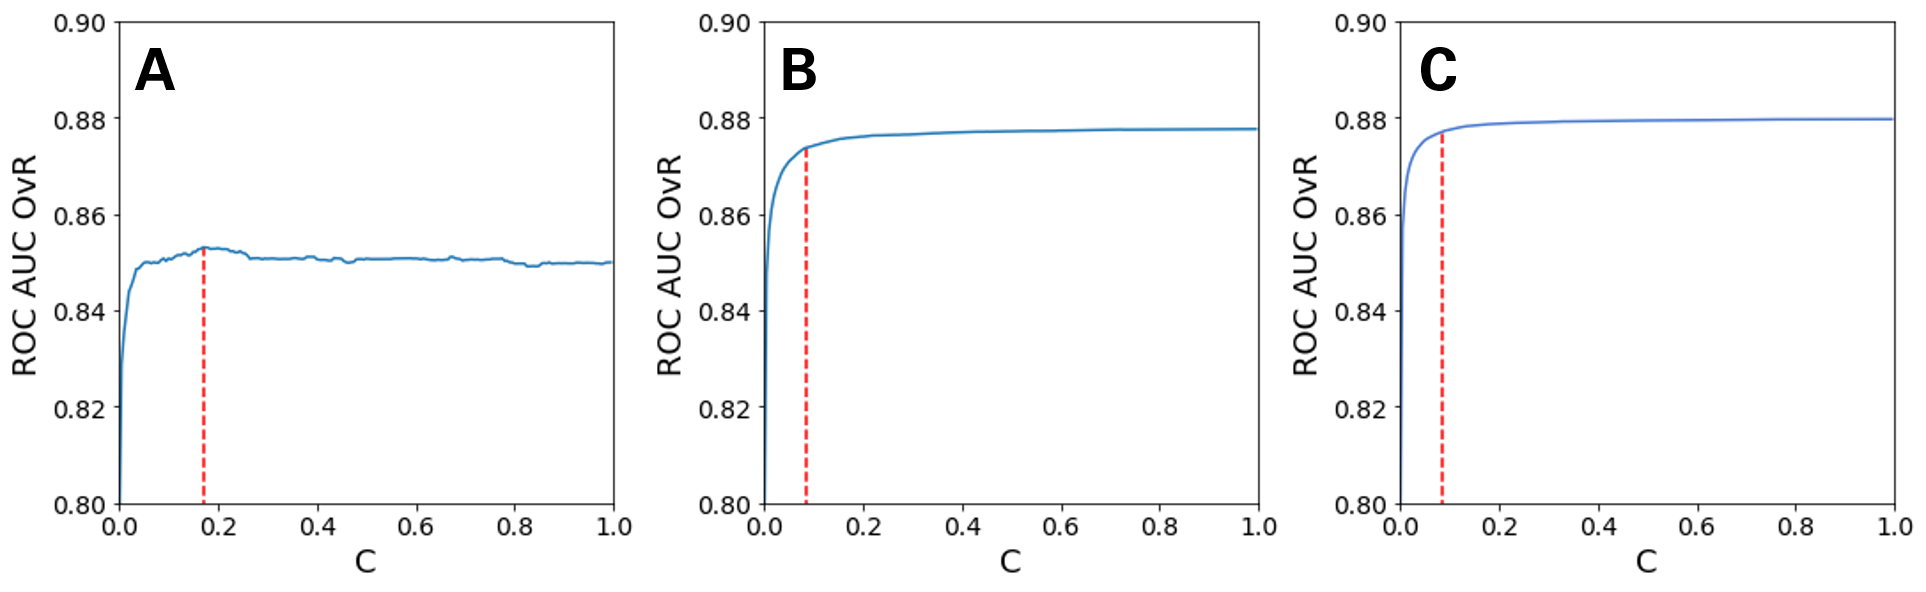
\includegraphics[width=\textwidth]{templates/images/Figure-LR_C_tuning.png}
\singlespacing
\caption[Logistic regression hyperparameter tuning]{Tuning plots for logistic regression C hyperparameter based on ROC AUC OvR values for A. WDS  B. WDS4 C. WDS8. WDS value selected from the plot maximum. Selections for WDS4 and WDS8 target the elbow of the curve.}
\label{fig:logreg_hp_tuning}
\end{figure}

The training and validation subsets defined in Section \ref{ch3:strat_sample} were re-combined, then stratified sampled as part of a 10-fold cross-validation process. ROC AUC OvR was used as the scoring metric. In some circumstances, a clear maximum can appear in cross-validation results indicating the best parameter choice, as is the case for WDS. For WDS4 and WDS8, AUC values continue to increase as C increases, but the slope of the AUC-C curve levels off to form a corner or “elbow” in the plot (Figure \ref{fig:logreg_hp_tuning}). Selecting a C value in this corner balances the trade-off between overfitting the training data with too little regularization and underfitting from too much regularization. The chosen C values for WDS, WDS4, and WDS8 are listed in Table \ref{tab:logreg_tuning}.

AUC values calculated on test subsets indicate WDS4 has the best out-of-sample performance of the three data sets. Figure \ref{fig:logreg_coefs} shows a plot of the feature coefficients for each of the one-vs-rest classifiers based on WDS4. Longer bars indicate larger influence on the model prediction. The top 5 features across the four classifiers are Si Geothermometer Temperature, Basement Depth, Drainage Density, Spring Density, and Volcanic Dike Density.

\begin{figure}[!htp]
\centering
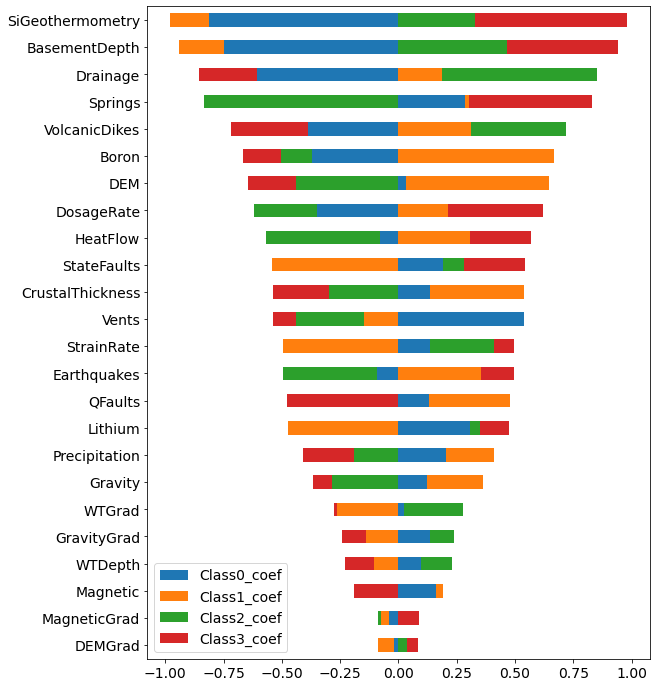
\includegraphics[width=\textwidth]{templates/images/Figure-LR-coefficients.png}
\singlespacing
\caption[Logistic regression feature coefficients]{Logistic regression coefficient values for OvR classifiers trained on WDS4.Stacked bar length is a proxy for overall importance to the classification.}
\label{fig:logreg_coefs}
\end{figure}

\subsubsection{Recursive Feature Elimination}
Logistic regression models assume a linear relationship between predictors and the response variable, but adding more predictors will not necessarily improve the model. Feature selection can lead to simpler models with the same predictive power but reduced risk of collinearity, which is important when managing data from naturally integrated earth systems. 

One method for selecting the number of features to keep involves an iterative process called \acrlong{rfe} (\acrshort{rfe}) (Brownlee, 2020c; scikit-learn, 2021d). The concept is relatively simple: RFE recursively selects and removes the feature with the smallest coefficient in the logistic regression model, then refits the data and repeats until a user-defined number of features is reached.  A plot of AUC vs. number of features can be constructed by looping over different feature limits, where the logistic regression model is fit on the training subset and evaluated on the validation subset (Figure \ref{fig:logreg_rfe}). Based on the plot, a local peak in AUC occurs when 18 features are used. Adding the remaining features results in small gains in AUC, but with diminishing returns for six additional features of complexity. Using this threshold, the data layers removed from the model include: DEM Gradient, Gravity Gradient, Magnetic Anomaly, Magnetic Anomaly Gradient, Water Table Depth, and Average Precipitation. Note that Average Precipitation appears higher on the coefficients plot (Figure \ref{fig:logreg_coefs}) than other features that were not removed. Since RFE iteratively removes predictors and refits the model, relative coefficients can change, particularly if there was collinearity with a removed variable.

\begin{figure}[!htp]
\centering
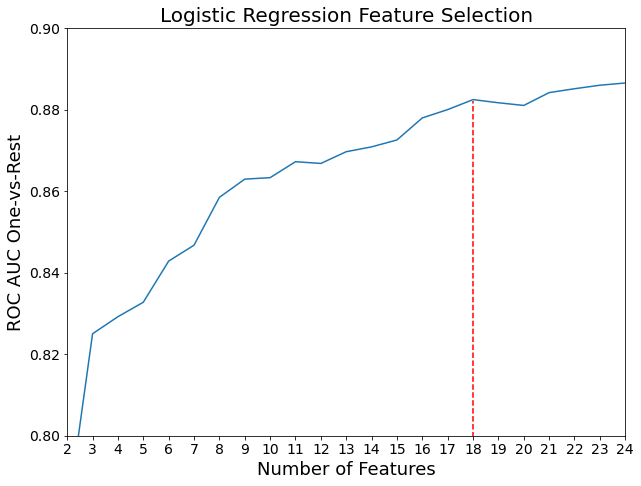
\includegraphics[width=0.6\textwidth]{templates/images/Figure-LR_feature_selection.png}
\singlespacing
\caption[Logistic regression feature selection]{Logistic regression feature selection using RFE and WDS4. Red dashed line indicates the chosen number of features to use for the LR model.}
\label{fig:logreg_rfe}
\end{figure}
\subsubsection{Optimized Model Results}\label{ch5:logreg_results}

\begin{wrapfigure}{R}{0.50\linewidth}
\centering
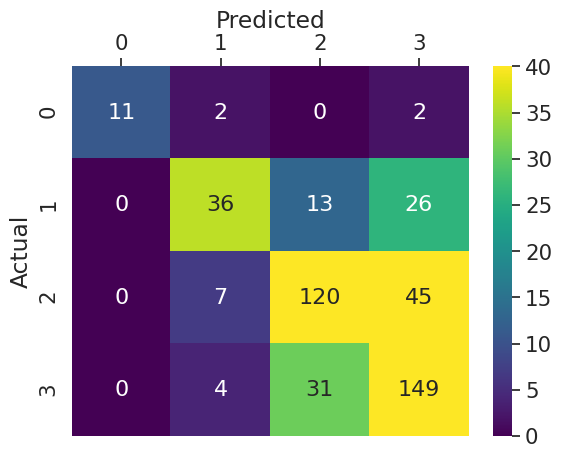
\includegraphics[width=0.45\textwidth]{templates/images/Figure-LR-ConfusionMatrix.png}
\singlespacing
\caption[Logistic regression confusion matrix]{Confusion matrix for the tuned LR model trained on WDS4.}
\label{fig:logreg_conf_matrix}
\end{wrapfigure}
A final LR model trained on WDS4 was constructed using the tuned C hyperparameter and reduced feature set from RFE. The confusion matrix suggests the model performs well overall (Figure \ref{fig:logreg_conf_matrix}). Correct predictions for all four classes of geothermal gradient (TP) outnumber the mis-classifications for those classes (FP). The model appears to struggle most with differentiating between class 2 and class 3 locations, which separate mid-grade (40-60 $^\circ$C/km) from high-grade gradients (>60 $^\circ$C/km), although there are a large number of mis-classifications (26) of low-grade gradient as high-grade as well.

Figure \ref{fig:logreg_auc} plots the macro average, micro average, and individual class ROC curves. Class 0 (non-thermal) predictive ability is quite high, pulling the micro-average AUC up to 0.88.  The macro AUC value of 0.85 is more aligned with the performance for other classes, which range from an AUC of 0.79-0.83. The trade-off between Class 2 and Class 3 is apparent in how the curve shapes mirror each other.

\begin{figure}[!htp]
\centering
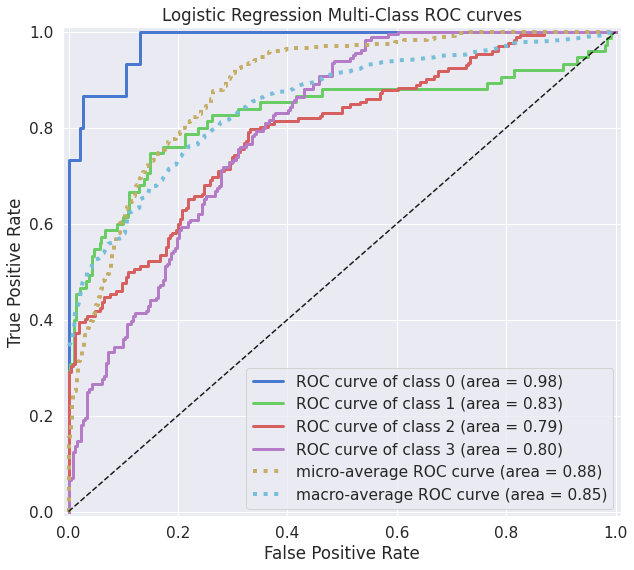
\includegraphics[width=0.6\textwidth]{templates/images/Figure-LR-AUC.png}
\singlespacing
\caption[Logistic regression AUC curves]{ROC AUC curves for the tuned LR model trained on WDS4.}
\label{fig:logreg_auc}
\end{figure}

Model predictions for the study area are generated by passing the FDS through the final trained model. Class predictions are plotted in Figure \ref{fig:logreg_final_map}. High-grade geothermal gradient patches are concentrated to the southeast and through the center of the AOI. Smaller high-grade regions are observed along the southwest state boundary, following the Rio Grande River to the northeast, and a smaller patch directly to the north.  Comparing this result to the data layer from \citet{bielicki_hydrogeolgic_2015}, high-grade predictions match in general spatial location except for the predicted patches to the north. The logistic regression model tends to predict more pervasive high geothermal gradients, and under-predicts the lower gradient regions to the north, east, and mid-AOI near the Rio Grande compared to the PFA layer.

\begin{figure}[!htp]
\centering
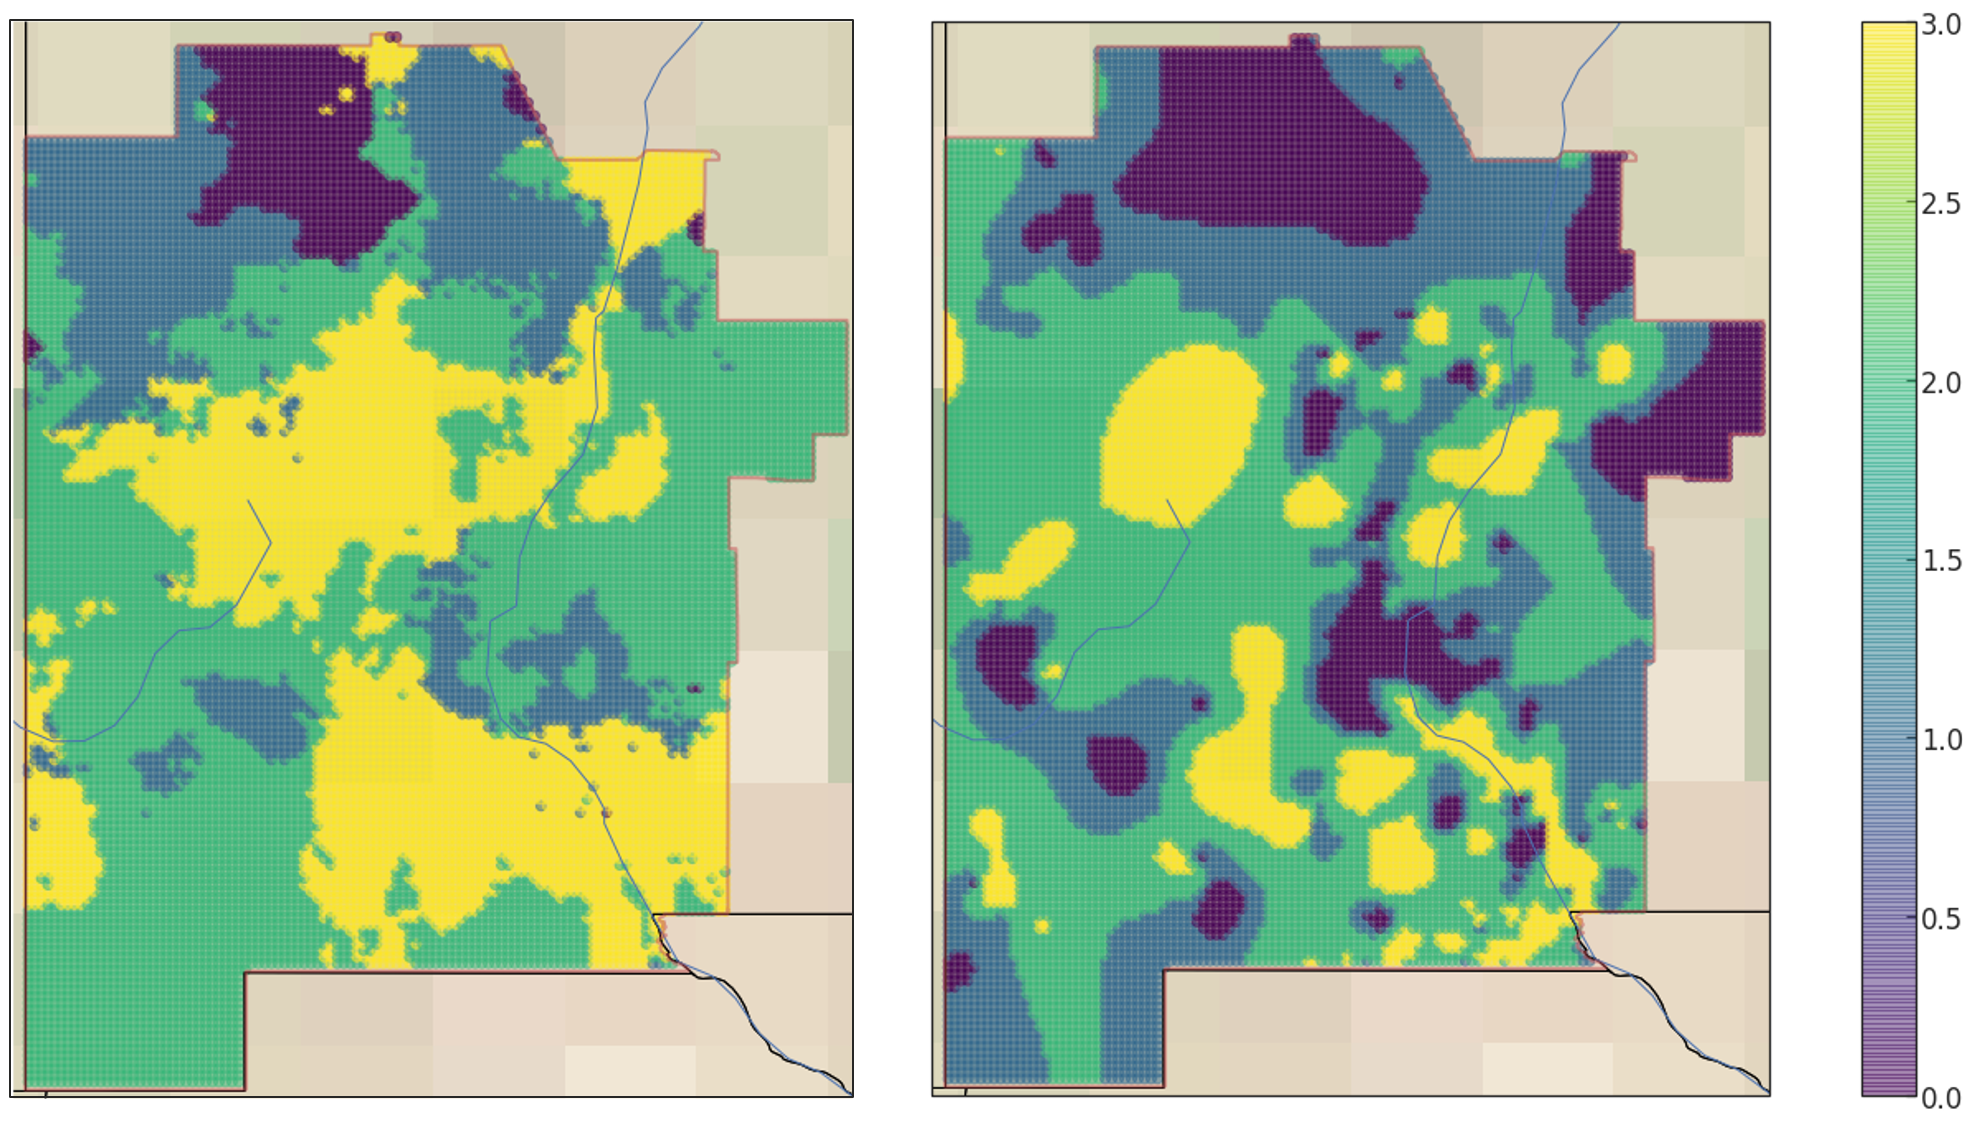
\includegraphics[width=\textwidth]{templates/images/Figure-LR-FinalMap_Joint.png}
\caption[Logistic regression prediction map]{Left: Map predictions of geothermal gradient class from the tuned LR model trained on WDS4. Right: geothermal gradient data layer from southwestern NM PFA study \protect\citep{bielicki_hydrogeolgic_2015}.}
\label{fig:logreg_final_map}
\end{figure}

\subsection{Decision Trees}\label{ch5:decision_trees}
 
A decision tree, sometimes known as a Classification and Regression Tree (CART), classifies observations using a cascading set of evaluations, each on individual predictor variables. There is no assumption of a linear response in the system. In fact, decision trees are uniquely suited to representing non-linear behavior in a highly-explainable way; once constructed, the decision tree describes a flowchart-like roadmap for each label assignment \citep[~p. 373-375]{bertsimas_analytics_2016}. Not every predictor will necessarily appear in the decision tree --- only those found to be significant during tree construction. And the most significant variables tend to be associated with early decision splits, placing them higher in the tree \citep[~p. 376]{bertsimas_analytics_2016}. Because of this, decision trees naturally provide insights into feature importance. 

\subsubsection{Tree Construction}
Decision trees are constructed by recursively performing binary splits on the training data set. Each split defines two new nodes in the tree, which correspondingly separates a group within the training data into subgroups. These subgroups represent child paths from the split node that terminate in two new terminal leaf nodes on the tree. The classification decision for each leaf will be the most commonly occurring class from the training data observations that are assigned to that leaf \citep[~p. 311]{james_introduction_2013}.

There are three metrics that can play a role in evaluating the discriminating quality of a particular decision node on the tree:

\begin{itemize}
    \item \textbf{Classification error rate}: the proportion of training samples that do not match the dominant class associated with a leaf node \citep[~p. 312]{james_introduction_2013}.
    \begin{equation} \label{eq:error_rate}
        E = 1 - \max_k(\hat{p}_{mk})
    \end{equation}
    where $m$ is the segment of the data associated with a node, $k$ is the class, and $\hat{p}_{mk}$ is the fraction of all training observations in $m$ that are of class $k$. 
    \item \textbf{Gini index}: measures variance across all k classes. Gini is sometimes known as a purity measurement because low values correspond with a strongly dominant class \citep[~p. 312]{james_introduction_2013}.
    \begin{equation}
        G = \sum_{k=1}^{K}{\hat{p}_{mk}(1-\hat{p}_{mk})}
    \end{equation}
    \item \textbf{Entropy}: An alternative form of purity measure, which also shows low values when the proportion of one class dominates the others within a node \citep[~p. 312]{james_introduction_2013}.
    \begin{equation}
        D = -\sum_{k=1}^{K}{\hat{p}_{mk}* \text{log}(\hat{p}_{mk})}
    \end{equation}
\end{itemize}

The purity aspect of both Gini index and entropy make them good choices for tree construction. In the forward pass, the tree will iteratively grow by selecting nodes in the tree, a predictor to split on, and a threshold value defining the split. These choices are optimized by the chosen quality metric. The tree will grow until a stopping condition is met, like reaching a maximum tree depth or minimum number of observations allowed per node. Tree clean-up then takes place in a backward pass, where the following decision tree objective governs whether a tree branch is kept or removed \citep[~p. 309]{james_introduction_2013}:

\begin{equation}
\min{\{SSE + \alpha\left|T\right|\}} = \min\Bigg\{ \sum_{m=1}^{\left|T\right|}{\sum_{i|x_i\epsilon R_m}}{(y_i-\hat{y}_m)^2+ \alpha\left|T\right|\Bigg\}}
\end{equation}

Here, $\left|T\right|$ refers to the number of terminal nodes in tree $T$, $R_m$ is the subgroup of the training data associated with terminal node $m$, and $\hat{y}_m$ is the classification predicted by node $m$. If the sum of squared errors ($SSE$) in classification increases by less than $\alpha$ when a branch is removed, that branch will remain removed from the decision tree. $\alpha$ acts as a regularization parameter balancing prediction accuracy with model complexity; greater values of $\alpha$ result in simpler decision trees.

\subsubsection{Hyperparameter Tuning}
Multiple hyperparameters determine the performance of a decision tree classifier. Here we consider six parameters, each of which are tuned using the Stratified k-Fold CV method described in Section \ref{ch5:strat_kfold_cv}, with 10 folds and the multi-class one-vs-rest ROC AUC as the scoring metric. The figure examples illustrate the tuning procedure for WDS4.

First, \verb|max_depth| and \verb|criterion| were tuned together. \verb|max_depth| limits tree expansion by capping the number of parameter evaluations (tree nodes) considered before a classification label assignment. \verb|criterion| refers to the quality metrics defined above. Figure \ref{fig:dtree_maxdepth} illustrates the relative insensitivity the classifier has to \verb|criterion|, while tree depth plays a stronger role in performance. A maximum AUC score is observed with a \verb|max_depth| of 8 and \verb|criterion| choice of Entropy.

\begin{figure}[!htp]
\centering
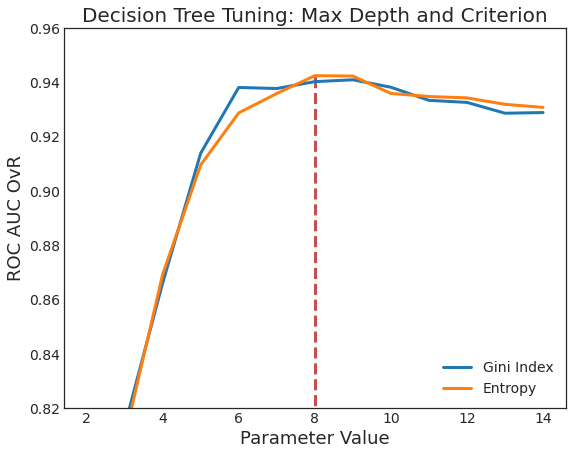
\includegraphics[width=.6\textwidth]{templates/images/Figure-DT_tuning_maxdepth_criterion.png}
\caption[Decision tree max depth tuning]{Results from stratified k-fold cross validation tuning of max\_depth and criterion hyperparameters using WDS4. The red dashed line indicates the selected max\_depth value.}
\label{fig:dtree_maxdepth}
\end{figure}

Next, \verb|min_samples_leaf| and \verb|min_samples_split| were tuned in succession. The former defines the minimum number of samples from the training set that must be assigned to a leaf node for that leaf to remain in the tree. The latter sets a minimum number of training set samples that must be assigned to a node before that node can be considered for a split. Figure \ref{fig:dtree_min_samples} illustrates the selected parameter values, defined by maxima in the AUC vs. parameter value plots. The insensitivity of the classifier to low values of \verb|min_samples_split| illustrates the cascading influence of the hyperparameters in this tuning flow. When \verb|min_samples_leaf| is set to 8, a split can only occur when the node being split has at least 16 observations, so any \verb|min_samples_split| value under 16 does not influence tree construction. 

\begin{figure}[!htp]
\centering
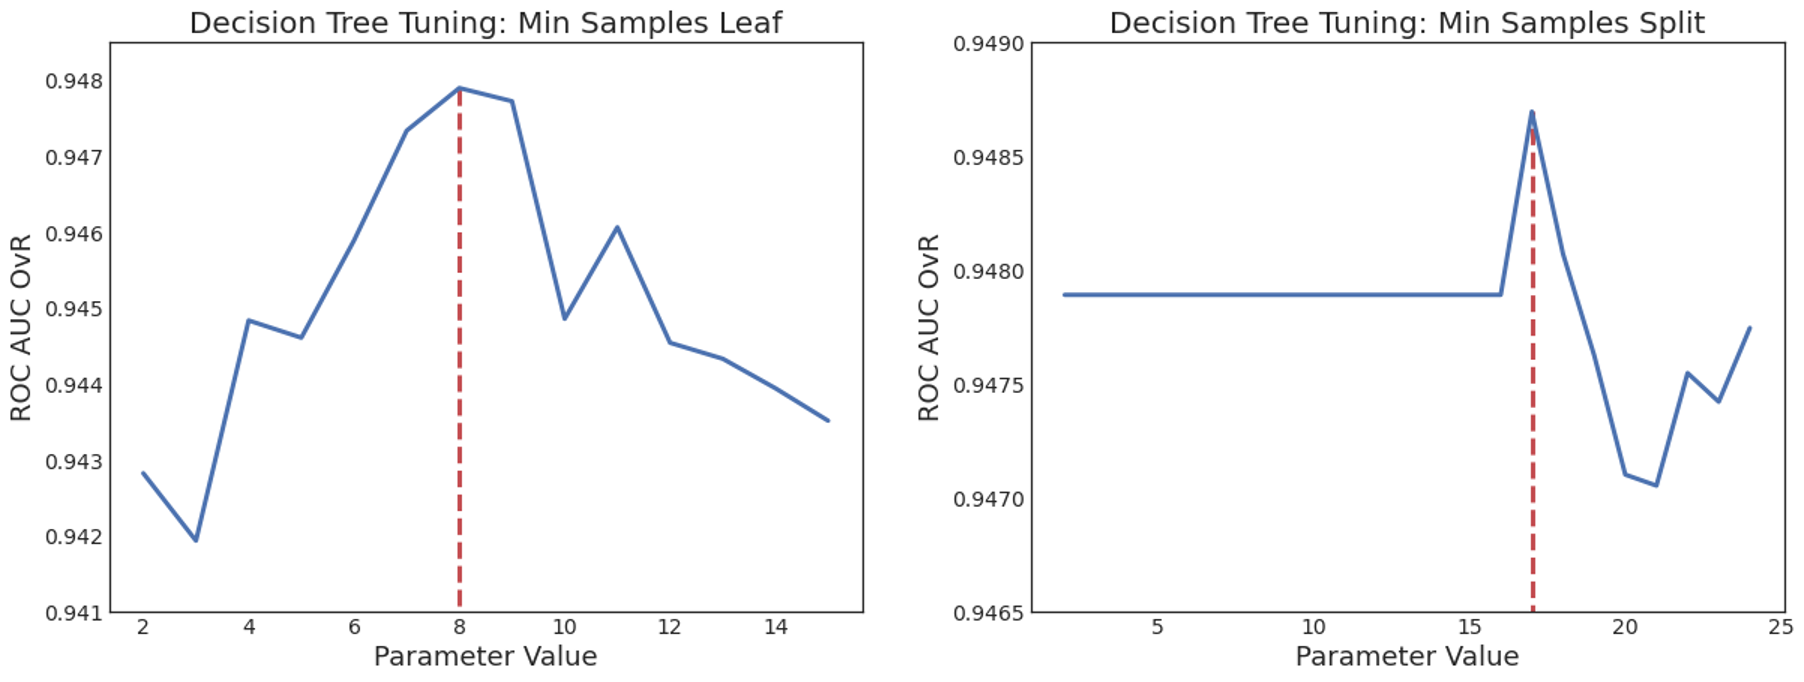
\includegraphics[width=\textwidth]{templates/images/Figure-DT_tuning_min_samp_leaf_split.png}
\caption[Decision tree min samples tuning]{Results from stratified k-fold cross validation tuning of min\_samples\_leaf (Left) and min\_samples\_split (Right) hyperparameters using WDS4. The red dashed lines indicate the selected values.}
\label{fig:dtree_min_samples}
\end{figure}

One optimization trick is to only consider a subset of the features when splitting decision tree nodes. This also adds an element of randomness to tree construction, so decision trees can differ when constructed on the same training data depending on how many features were considered for each split. No clear maximum appears in the AUC plot for \verb|max_features| (Figure \ref{fig:dtree_max_features}), so a value of 8 was selected using the elbow criterion described in Section \ref{ch5:hyper_tuning}. \verb|max_features| can also cause problems when performing feature selection if the feature count drops  below the \verb|max_features| value, so care must be taken in using this parameter.

\begin{figure}[!htp]
\centering
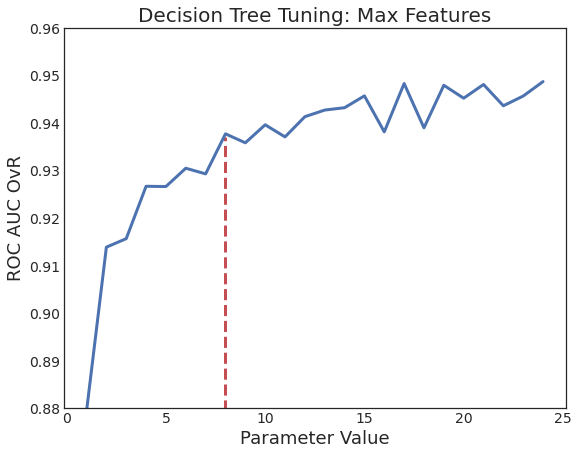
\includegraphics[width=.6\textwidth]{templates/images/Figure-DT_tuning_max_features.png}
\caption[Decision tree max features tuning]{Results from stratified k-fold cross validation tuning of max\_features parameter using WDS4. The red dashed line indicates the selected value, selected in the “elbow” of the plot.}
\label{fig:dtree_max_features}
\end{figure}

The final parameter, \verb|ccp_alpha|, controls the trade-off between model fit and complexity during the tree pruning backward pass of tree construction. As the alpha value increases from zero, the difference between in-sample (training) and out-of-sample (validate) performance decreases, but so does the overall performance of the classifier on the validation subset. Figure \ref{fig:dtree_alpha} shows a clear minima in train-validate AUC difference, however the validation set performance drops from 0.95 to under 0.85 when using this value for \verb|ccp_alpha|. The default value of \verb|ccp_alpha| = 0.0 is chosen instead.

\begin{figure}[!htp]
\centering
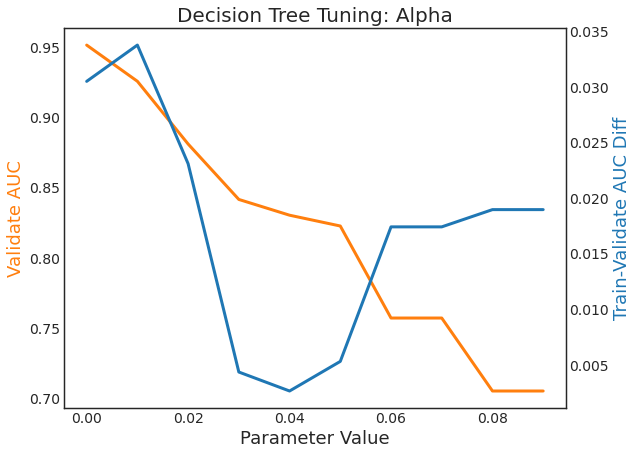
\includegraphics[width=.6\textwidth]{templates/images/Figure-DT_tuning_alpha.png}
\caption[Decision tree alpha tuning]{Results from stratified k-fold cross validation tuning of the ccp\_alpha parameter. The orange line plots the validation subset AUC. The blue line plots the difference in AUC between training and validation subsets.}
\label{fig:dtree_alpha}
\end{figure}

Final hyperparameter values and performance results for WDS, WDS4, and WDS8 are listed in Table \ref{tab:dtree_tuning}. Data augmentation results in a significant improvement in classifier performance over the original WDS.

\begin{table}[!htp]
\centering
\begin{tabular}{c|c|c|c|}
\cline{2-4}
                                          & WDS & WDS4 & WDS8 \\ \hline
\multicolumn{1}{|c|}{criterion}           & Gini & Entropy & Entropy \\ \hline
\multicolumn{1}{|c|}{max\_depth}          & 5 & 8 & 10 \\ \hline
\multicolumn{1}{|c|}{min\_samples\_leaf}  & 7 & 8 & 10 \\ \hline
\multicolumn{1}{|c|}{min\_samples\_split} & 21 & 17 & 24 \\ \hline
\multicolumn{1}{|c|}{max\_features}       & 5 & 8 & 6 \\ \hline
\multicolumn{1}{|c|}{ccp\_alpha}          & 0  & 0 & 0 \\ \hline
\multicolumn{1}{|c|}{AUC$_{train}$}       & 0.89 & 0.97 & 0.99 \\ \hline
\multicolumn{1}{|c|}{AUC$_{test}$} & 0.82 & 0.95 & 0.96 \\ \hline
\end{tabular}
\caption[Decision tree hyperparameter values]{Tuned hyperparameter selections and resulting model AUC for training and test subsets of WDS, WDS4, and WDS8.}
\label{tab:dtree_tuning}
\end{table}

Figure \ref{fig:dtree_feat_import} shows the feature importances determined by the decision trees for WDS, WDS4, and WDS8.  Features are sorted on the sum importance value across all 3 data sets. Although differences exist, Si Geothermometer Temperature appears as the most important predictor in all cases. And the bottom six features are also remarkably consistent across the data sets: Water Table Depth, Water Table Gradient, Gravity Anomaly Gradient, Magnetic Anomaly, Magnetic Anomaly Gradient, and DEM Gradient. Dropping these features reduces the overall decision tree data set to 18 features total.

\begin{figure}[!htp]
\centering
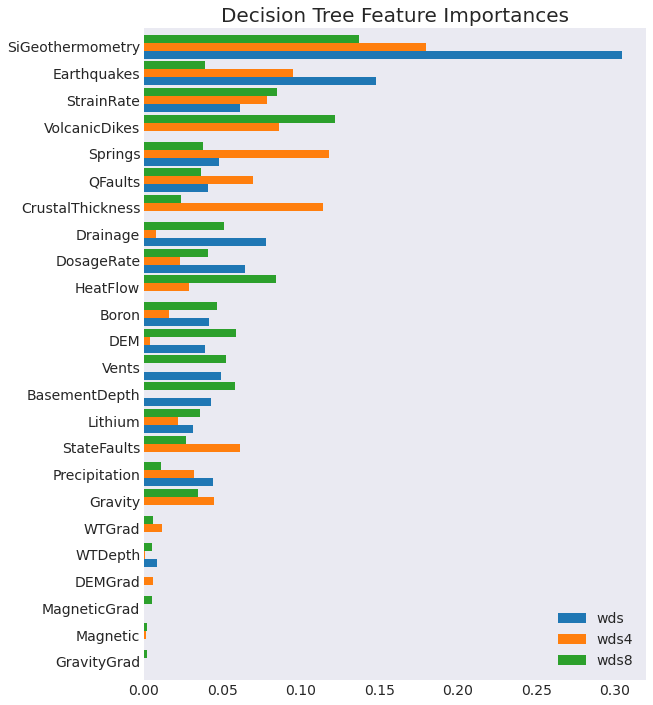
\includegraphics[width=\textwidth]{templates/images/Figure-DT_feature_importances_all.png}
\caption[Decision tree feature importances]{Decision tree feature importances for WDS, WDS4, and WDS8, sorted on the sum total importance across the 3 data sets.}
\label{fig:dtree_feat_import}
\end{figure}

\subsubsection{Optimized Model Results}
\begin{figure}[!htp]
\centering
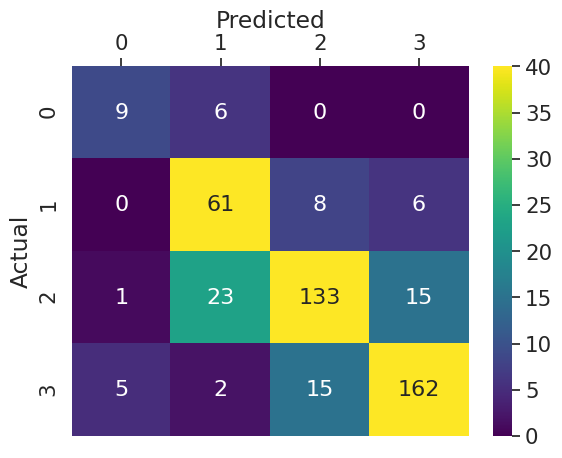
\includegraphics[width=0.45\textwidth]{templates/images/Figure-DT-ConfusionMatrix.png}
\singlespacing
\caption[Decision tree confusion matrix]{Confusion matrix for tuned DT model trained on WDS4.}
\label{fig:dtree_conf_matrix}
\end{figure}
A final DT model trained on WDS4 was constructed using the tuned parameters and 18-predictor reduced feature set. The confusion matrix (Figure \ref{fig:dtree_conf_matrix}) demonstrates an improvement in model results over the logistic regression method. Low-grade geothermal locations are correctly predicted for almost double the number of sites, and half as many mis-classifications are observed between class 2 (mid-grade) and class 3 (high-grade) geothermal as with the LR model.

Figure \ref{fig:dtree_auc} shows the macro average, micro average, and individual class DT ROC curves. All individual class AUC values exceed 0.90. Class 0 (non-geothermal) continues to demonstrate the highest predictive ability (AUC=0.97), but the performance of class 3 (high-grade) is most responsible for boosting micro-average AUC at higher decision thresholds where the class 0 ROC curve steeply drops in TPR for FPR < 0.1. Class 2 (medium-grade) classification performance lags behind the other classes for the DT classifier.

\begin{figure}[!htp]
\centering
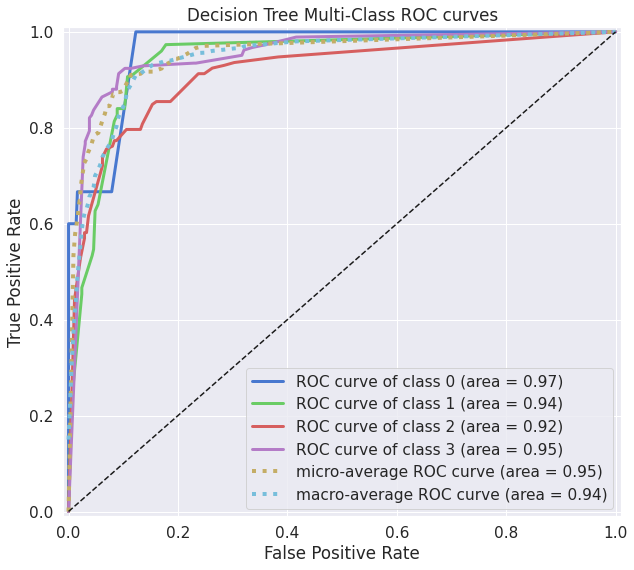
\includegraphics[width=0.6\textwidth]{templates/images/Figure-DT_AUC.png}
\caption[Decision tree AUC curves]{ROC AUC curves for the tuned DT model trained on WDS4.}
\label{fig:dtree_auc}
\end{figure}

Model predictions for the study area are generated by passing the FDS through the DT model. Class predictions based on the OvR methodology are plotted in Figure \ref{fig:dtree_final_map}. The high-grade geothermal gradient patches to the southeast and central regions of the AOI are smaller in areal extent and more disconnected than for the LR model (Figure \ref{fig:logreg_final_map}). Predictions for low or no-gradient are concentrated to the NW in the CP province, central-east where RGR transitions into the Great Plains, and south in the southern BR province. The overall distribution of geothermal gradient classes matches the \citet{bielicki_hydrogeolgic_2015} PFA layer (Figure \ref{fig:dtree_final_map}) with a greater distribution of high-gradient locations and fewer low/no-gradient ones.

\begin{figure}[!htp]
\centering
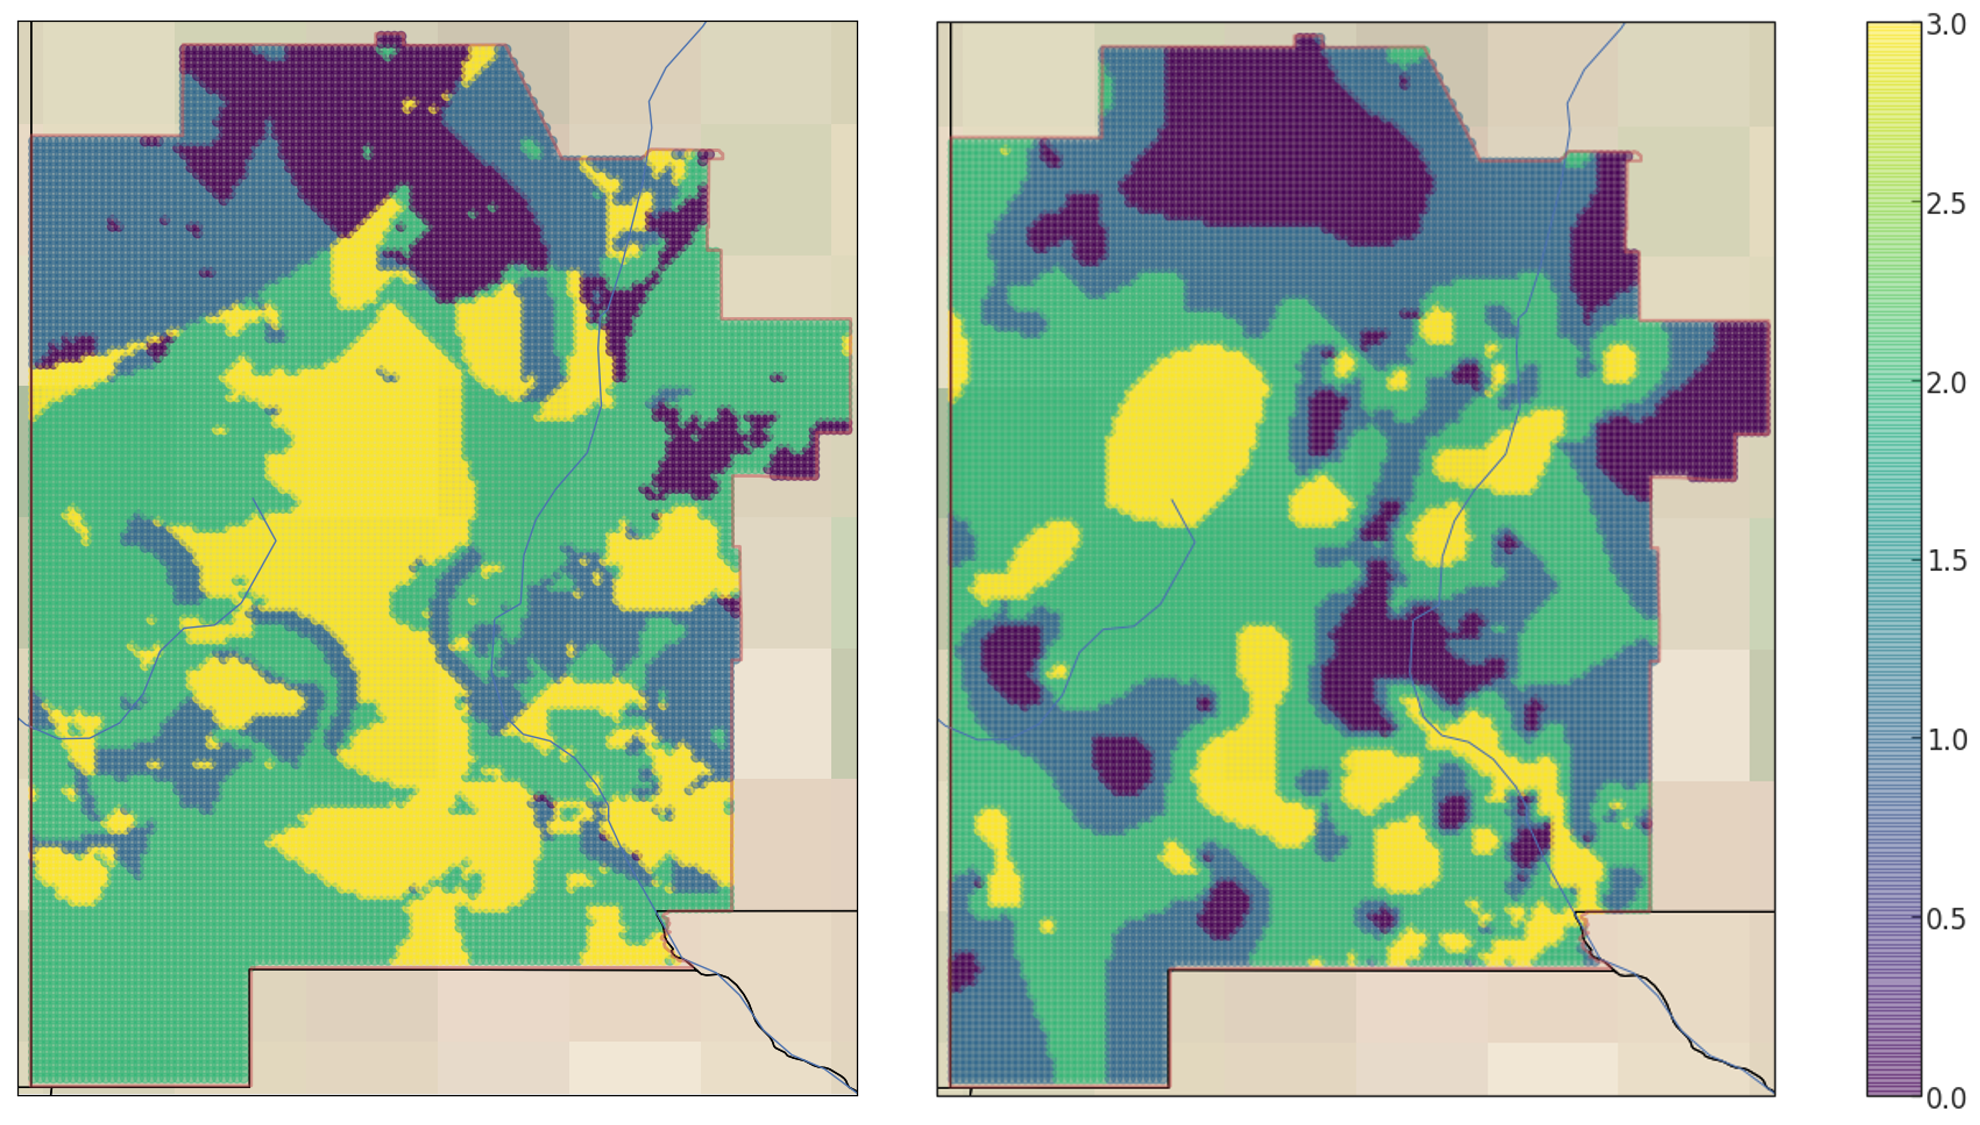
\includegraphics[width=\textwidth]{templates/images/Figure-DT-FinalMap_Joint.png}
\caption[Decision tree prediction map]{Left: Map predictions of geothermal gradient class from the tuned DT model trained on WDS4. Right: geothermal gradient data layer from southwestern NM PFA study \protect\citep{bielicki_hydrogeolgic_2015}}
\label{fig:dtree_final_map}
\end{figure}

Interesting high-gradient patches appear to the southwest and northeast, one of which is surrounded by an unusually cohesive ring of class 0 non-thermal predictions. Note that when the random seed changes and a new decision tree is constructed, this ring typically goes away. In fact, one downside of the decision tree model is its unstable nature; decision trees can change each time the algorithm is run, even on the same training data, due to randomness in the node splitting process. Nevertheless, tree performance remains relatively stable overall. And the ability to plot and trace through the model makes it one of the most accessible and interpretable methods to use (See Figure \ref{fig:dtree_viz}).

\begin{figure}[!htp]
\centering
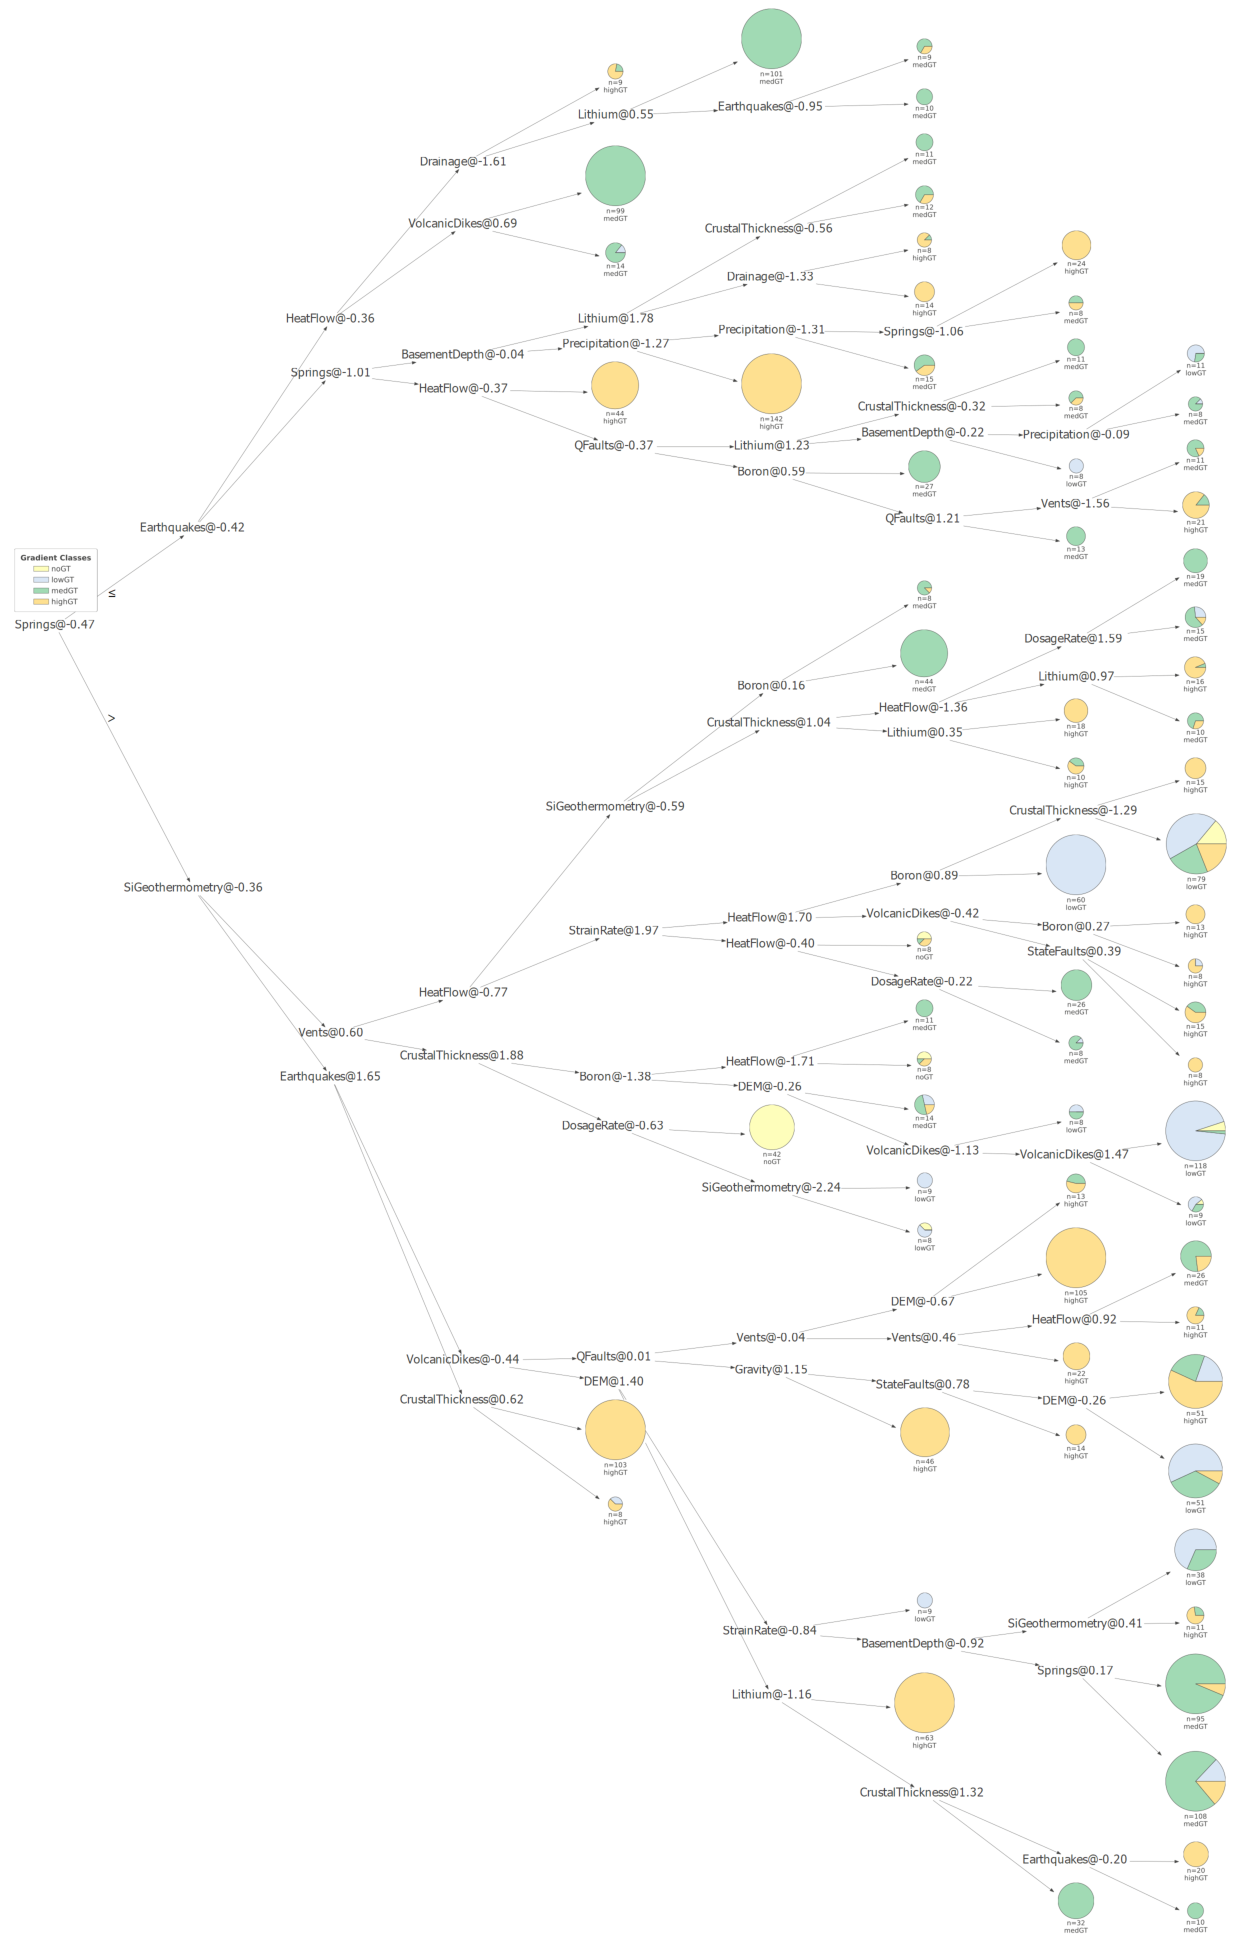
\includegraphics[height=0.9\textheight,keepaspectratio]{templates/images/Figure-DT_viz_portrait.pdf}
\caption[Decision tree visualization]{Decision tree visualization for the final decision tree model.Nodes are noted by predictor labels with their decision threshold. Bubbles illustrate the final distribution of classes in a leaf node, sized by number of observations. The majority class determines the classification label.}
\label{fig:dtree_viz}
\end{figure}

\subsection{Tree Ensembles}

\subsection{Neural Networks}

\subsection{Uncertainty Analysis}

\subsubsection{Bootstrap Estimation}

\subsubsection{Information Entropy}

\subsubsection{Bayesian Networks}
